\section{Turbulence IV}

\subsection{Review: The double cascade}

\begin{center}
    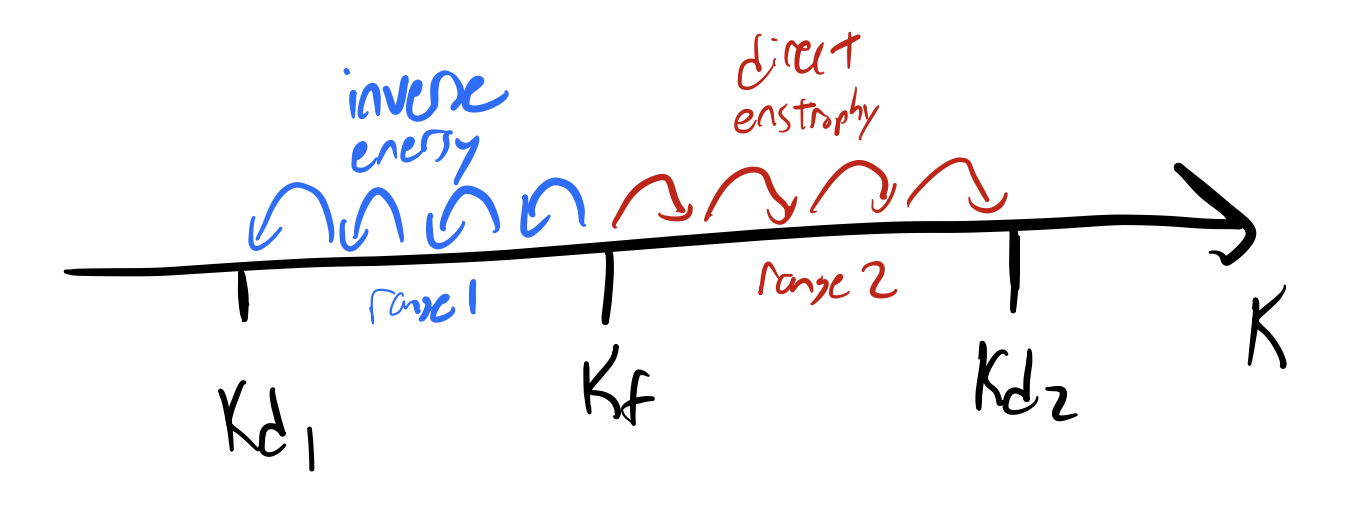
\includegraphics[scale=0.4]{Lectures/Images/lec15-dualcascade.png}
\end{center}

Between $k_{d_1}$ and $k_{d_2}$, we have an inertial regime with no dissipation. We considered two scenarios where we injected energy at $k_f$. Then we found that there is an inverse energy cascade towards $k_{d_1}$ and a direct enstrophy cascade towards $k_{d_2}$. The enstrophy was defined as the integral of vorticity:
\begin{equation}
    Z = \int \gv{\omega}^2 d^2\v{x}.
\end{equation}

The argument was derived by Kraichnan 1967, who started looking at nonlinear PDEs by studying gravity at IAS with Einstein. He then turned to turbulence, and did the rest of his academic career as a hermit living in a cabin in New Hampshire.

\subsection{Power Spectrum Derivation}
We now have the direction of the cascade - let us now figure out the power spectrum, in the same way that we derived the power spectrum for the energy cascade in the Kolmogorov argument.

Note that there is an important implicit assumption, namely that of locality (in $k$-space). More precisely, we assume that non-local energy transfer between far-away $k$ values is not possible, and hence the spectrum in range 1 only depends on the the rate of energy injection $\e$, and the spectrum in range 2 only depends only on the rate of enstrophy production $\eta$. Hence, in $k$-space we can treat the two problems as independent. Note that $\eta = k^2\e$ so we are not saying that there is only energy or enstrophy in one of the two regimes, just that there is a dominant process (and hence energy spectrum power law) in each regime.

First, let's look at the dimensionality of $\eta$:
\begin{equation}
    [\eta] = \frac{[\text{enstrophy density}]}{[\text{time}]} = \frac{[\gv{\omega}^2]}{[t]} = \frac{[(\nabla \times \v{v})^2]}{[t]} = \frac{\left(\frac{1}{[t]}\frac{[L]}{[t]}\right)^2}{[t]} = \frac{1}{[t]^3}
\end{equation}
The dimensionality of $E_k$ (power spectrum of energy) is:
\begin{equation}
    [E_k] = \frac{[l]^3}{[t]^2}
\end{equation}
So we want a relation:
\begin{equation}
    E_k = c_2\eta^{\alpha}k^{\beta}
\end{equation}
$\eta$ provides the time dependence, $k$ provides the spatial dependence, so:
\begin{equation}
    E_k = c_2\eta^{2/3}k^{-3}
\end{equation}
The argument for the direct cascade we did a couple lectures ago (Kolmogorov '41) yielded:
\begin{equation}
    E_k = c_1\e^{2/3}k^{-5/3}
\end{equation}
so we have two power laws, which dominate in different regimes.

\subsection{Turbulence + Odd Viscosity}
We now want to study what happens when we add odd viscosity - e.g. a rotating box/atmosphere, or individually rotating particles. This leads to a quasi-2-dimensionalization of the fluid flow.

In 3D we would expect to have a picture where we have a soup\footnote{You shouldn't eat it.} of vortices in 3D which is scale invariant in the cascading regime. What we will see happen is that we still will have many vortices, but they will be roughly aligned along the direction $\hat{\gv{\Omega}}$ of rotation.

\begin{center}
    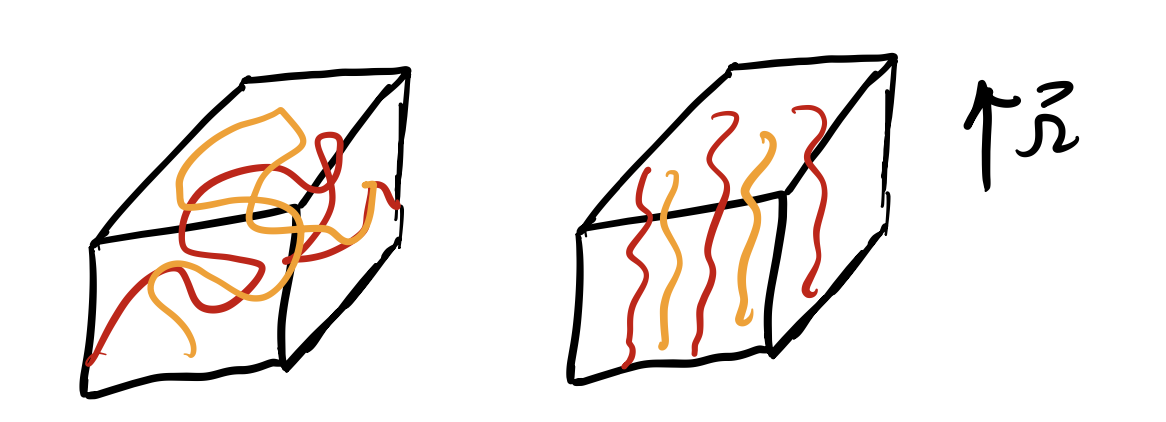
\includegraphics[scale=0.4]{Lectures/Images/lec15-vortices.png}
\end{center}

Let's return to the Navier-Stokes equation, adding a rotation term
\begin{equation}
    \p_t \v{v} + \v{v} \cdot \nabla \v{v} = -\frac{1}{\rho_0}\nabla p + \nu\nabla^2\v{v} + \begin{cases}
        \Omega \hat{\v{z}} \times \v{v} & \text{Coriolis} \\ \nu^0 \hat{\v{z}} \times \nabla^2 \v{v} & \text{Odd Viscosity}
    \end{cases}
\end{equation}
with $\nu = \eta/\rho$. Notice that, comparing the two cases, we can interpret odd viscosity as a length scale dependent coriolis force $\sim \Omega v \nu^0 k^2$.

\subsection{Taylor-Proudman Argument}
The following argument is presented by Proudman and G.I. Taylor, who is famous for estimating the energy of the Trinity nuclear test to the correct order of magnitude. 

We have two dimensionless parameters of interest; the Reynolds number $\text{Re} = \frac{VL}{\eta}$ and the odd viscosity ratio $\frac{\nu^0}{\nu}$. The $\frac{\nu^0}{\nu} \ll 1$ case is ``simple'', we can drop the $\nu^0$ term and then this is just isotropic viscosity, and we already know the power spectrum to be $\sim k^{-5/3}$ (this the Kolmogorov regime). The interesting limit is $\frac{\nu^0}{\nu} \gg 1$. The argument relies on a balance between two terms, the pressure and the rotational term. We neglect the $\v{v} \cdot \nabla \v{v}$ term - this is ok for low Reynolds, but is problematic at high Reynolds.

Let's look at the argument for the odd viscosity case. The balance of the term gives us:
\begin{equation}
    \eta^0 \hat{\v{z}} \times \nabla^2\v{v} = \nabla p
\end{equation}
Let us now take a curl on both sides, wherein the pressure term vanishes (curl of grad is zero). Now, we use the identity:
\begin{equation}
    \nabla \times (\v{F} \times \v{G}) = \v{F}\nabla \cdot \v{G} - \v{G}\nabla \cdot \v{F} + (\v{G} \cdot \nabla)\v{F} - (\v{F}\cdot\nabla)\v{G}
\end{equation}
where we have $\v{F} = \zhat$ and $\v{G} = \nabla^2\v{v}$. Since $\zhat$ is a constant, the derivative terms of $\zhat$ vanish (so the second/third terms drop out). Further, the first term drops out as:
\begin{equation}
    \nabla \cdot (\nabla^2\v{v}) = \nabla^2(\nabla \cdot \v{v}) = 0
\end{equation}
from incompressibility. Hence we are left with:
\begin{equation}
    \eta^0(\zhat \cdot \nabla)\nabla^2\v{v} = 0 \implies  \nabla^2\p_z\v{v} = 0
\end{equation}
This tells us that:
\begin{equation}
    \boxed{\p_z \v{v} \approx \v{0}}
\end{equation}
This is the sense that we believe that there might be quasi-2-dimensionalization.

\subsection{Regimes of Turbulence}
This was a fairly simple and approximate argument. But, one thing we can do is also simulate the Navier-Stokes equations with the odd viscosity term, and observe what we see. 

\begin{center}
    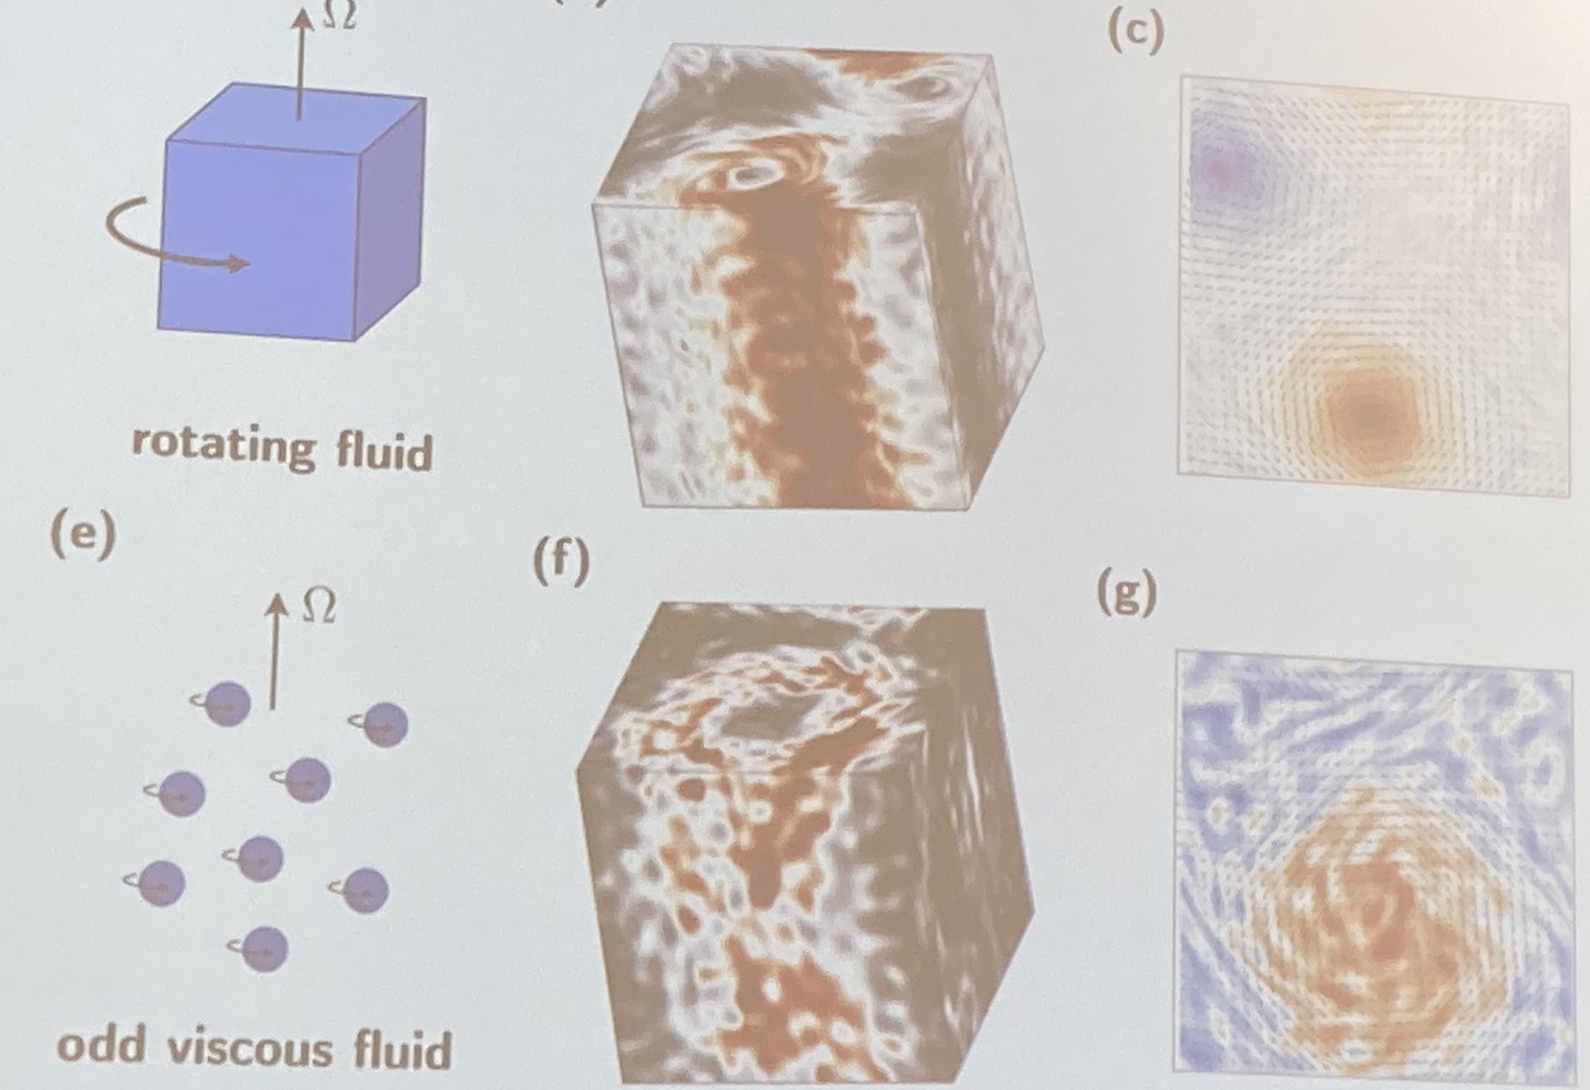
\includegraphics[scale=0.4]{Lectures/Images/lec15-simulation.png}
\end{center}

We notice that for the most part, we have a column vortex in the $\zhat$ direction\footnote{Why is the quasi-2-dimensionalization harder to see in the odd viscous fluid case? We have to go to high $k$ so that the odd viscosity effect is important. There's a subtlety because the vortices are on the length scale of the box, while they are caused by small-scale physics (rotating particles), so there is a lot of information to retain - it (unlike the Coriolis/body force case) is a multiscale problem.}, which is what the Taylor-Proudman argument hints at. But this simulation is done in a regime where the $\v{v} \cdot \nabla \v{v}$ term is kept - there are mathematical arguments that nonlinearities introduced by this term do not spoil the quasi-2-dimensionalization.

Note that when comparing the rotating fluid and odd viscosity case, we have the $k^2$ length-scale dependence. If $k$ is very small (no matter how large $\nu^0$ is) then the odd viscosity term drops out and we just have Kolmogorov turbulence, with a forward energy cascade and energy spectrum that scales as $\sim k^{-5/3}$. At large $k$ the odd viscosity term becomes important, and we have quasi-2-dimensionalization, wherein we have an inverse cascade. The two asymptotic regimes are separated by a characteristic inverse wavelength $k_{\text{odd}}$ representing the crossover between the two regimes. So, there are two things to try to find - the power spectrum scaling as well as the crossover wavelength (and what happens in this regime).

\begin{center}
    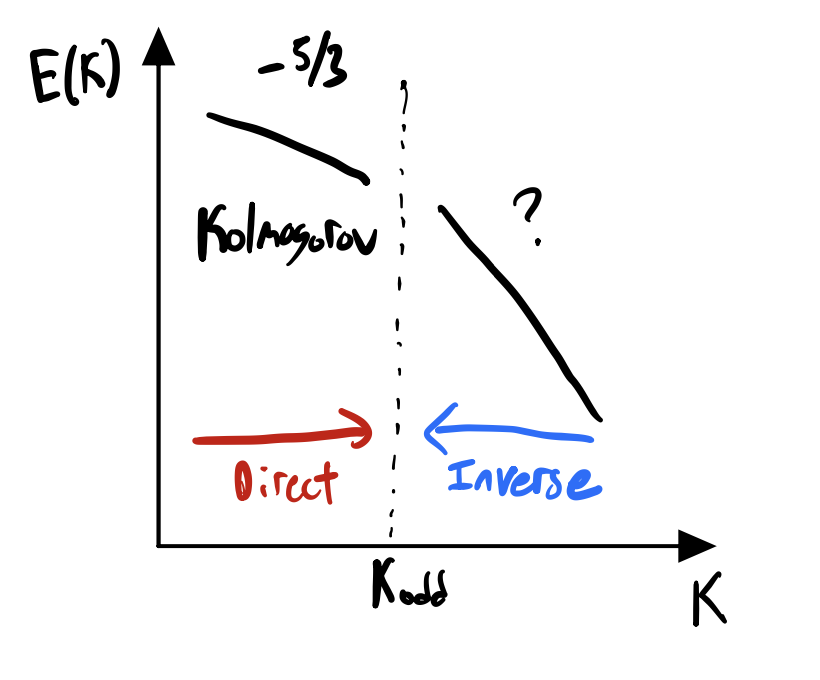
\includegraphics[scale=0.4]{Lectures/Images/lec15-oddpowerspectrum.png}
\end{center}

It is interesting to compare this with the Kraichnan argument, where we have an outward flux of energy/enstrophy away from $k_f$, vs. here where we have an inward flux of energy towards $k_{\text{odd}}$. In $k$-space we expect a sharp peak at $k_{\text{odd}}$ which suggests that there is a periodic behaviour of the system in real space.

One thing we can say is that $k_{\text{odd}} \sim f(\nu^0)$, because $\nu^0 = 0$ then $k_{\text{odd}}$ would be infinity (we would just have the Kolmogorov turbulence at all scales).

Let's start by estimating the power spectrum power law (we make the physical assumption that $\e$ is linear in the characteristic time $\tau$ - this is not physically obvious)
\begin{equation}
    \e = A\tau k^\alpha E^\beta(k)
\end{equation}

We know that $[\tau] = t$, $[\e] = \frac{l^2}{t^3}$ and $[E(k)] = \frac{l^3}{t^2}$. So:
\begin{equation}
    [\e] = l^{-\alpha + 3\beta} t^{-2\beta + 1} \implies l^2 t^{-4} = l^{-\alpha + 3\beta}t^{-2\beta}
\end{equation}
hence:
\begin{equation}
    2 = 3\beta - \alpha
\end{equation}
\begin{equation}
    -4 = -2\beta
\end{equation}
which is solved by:
\begin{equation}
    \beta = 2, \alpha = 4
\end{equation}

So by dimensional analysis, we find:
\begin{equation}
    \boxed{\e = A\tau(k)k^4 E^{2}(k)}
\end{equation}
which tells us that if we know the characteristic time scale of our process and the power spectrum, we know the energy transfer rate. We can then invert this to obtain an equation of the power spectrum in terms of $\e, \tau, k$. If we put the Eddy turnover time in for $\tau$ then we get the Kolmogorov result, and we will make an appropriate modification for the odd turbulence case.

For more detail, you may refer to \texttt{De Wit, Fruchart, Khain, Toschi, Vitelli, \emph{Nature 2024}}.


Next time, we will also study how linear stability analysis can be used to study pattern formation. This is something we will look at next lecture. What is very interesting to note here is that we have a very different mechanism of pattern formation, via energy cascades from turbulence (highly nonlinear)! 